\documentclass[tikz,border=10pt]{standalone}
\usepackage{tikz}
\usetikzlibrary{shapes.geometric, arrows.meta, positioning}

\tikzset{
    register/.style={
        rectangle, draw=black, thick,
        minimum width=0.9cm, minimum height=0.75cm,
        fill=white, font=\small\ttfamily
    },
    alu/.style={
        rectangle, draw=black, thick,
        minimum width=0.85cm, minimum height=0.65cm,
        fill=white, font=\small
    },
    wire/.style={draw=black, thick, -Stealth},
    buswidth/.style={font=\tiny, fill=white, inner sep=1pt},
    logic/.style={
        rectangle, draw=black, thick, rounded corners=3pt,
        minimum width=0.75cm, minimum height=0.65cm,
        fill=gray!10, font=\small
    }
}

\begin{document}
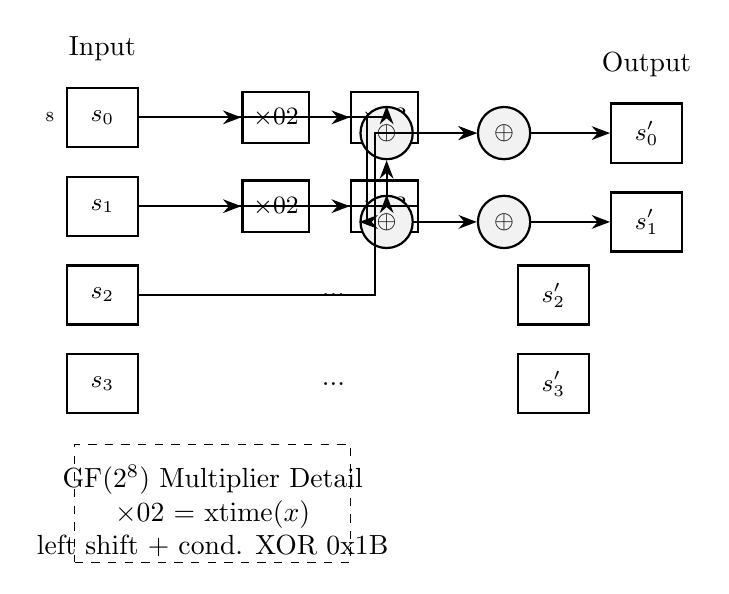
\begin{tikzpicture}[node distance=0.7cm and 1cm]

% Input bytes
\node[register] (s0) at (0,0) {$s_0$};
\node[register, below=0.35cm of s0] (s1) {$s_1$};
\node[register, below=0.35cm of s1] (s2) {$s_2$};
\node[register, below=0.35cm of s2] (s3) {$s_3$};

\node[font=\normalsize, above=0.2cm of s0] {Input};
\node[buswidth, left=0.1cm of s0] {8};

% GF multipliers (first two rows)
\node[alu, right=1.3cm of s0] (m02_0) {$\times$02};
\node[alu, right=0.5cm of m02_0] (m03_0) {$\times$03};

\node[alu, right=1.3cm of s1] (m02_1) {$\times$02};
\node[alu, right=0.5cm of m02_1] (m03_1) {$\times$03};

\draw[wire] (s0) -- (m02_0);
\draw[wire] (s0.east) -- ++(0.4,0) |- (m03_0);
\draw[wire] (s1) -- (m02_1);
\draw[wire] (s1.east) -- ++(0.4,0) |- (m03_1);

% XOR trees (first two outputs)
\node[logic, circle, minimum size=0.6cm, right=2.8cm of s0, yshift=-0.2cm] (x0a) {$\oplus$};
\node[logic, circle, minimum size=0.6cm, right=0.8cm of x0a] (x0b) {$\oplus$};

\node[logic, circle, minimum size=0.6cm, right=2.8cm of s1, yshift=-0.2cm] (x1a) {$\oplus$};
\node[logic, circle, minimum size=0.6cm, right=0.8cm of x1a] (x1b) {$\oplus$};

\draw[wire] (m02_0) -| (x0a);
\draw[wire] (m03_1) -| (x0a);
\draw[wire] (x0a) -- (x0b);
\draw[wire] (s2.east) -- ++(3,0) |- (x0b);

\draw[wire] (m02_1) -| (x1a);
\draw[wire] (s0.east) -- ++(2.9,0) |- (x1a);
\draw[wire] (x1a) -- (x1b);

% Output bytes
\node[register, right=1cm of x0b] (o0) {$s_0'$};
\node[register, right=1cm of x1b] (o1) {$s_1'$};
\node[register, right=4.8cm of s2] (o2) {$s_2'$};
\node[register, right=4.8cm of s3] (o3) {$s_3'$};

\draw[wire] (x0b) -- (o0);
\draw[wire] (x1b) -- (o1);

\node[font=\normalsize, right=2.2cm of s2] {...};
\node[font=\normalsize, right=2.2cm of s3] {...};

\node[font=\normalsize, above=0.2cm of o0] {Output};

% GF multiplier detail box
\node[draw, dashed, below=1.5cm of s2, minimum width=3.5cm, minimum height=1.5cm, xshift=1.4cm] (detail) {};
\node[font=\normalsize, below=0.15cm of detail.north] {GF($2^8$) Multiplier Detail};
\node[font=\normalsize, below=0.6cm of detail.north, align=center] {$\times$02 = xtime($x$)\\left shift + cond. XOR 0x1B};

\end{tikzpicture}
\end{document}
